\def\baselinestretch{1}
\chapter{Discussion}
\ifpdf
    \graphicspath{{discussion/discussion-figs/PNG/}{discussion/discussion-figs/PDF/}{discussion/discussion-figs/}}
\else
    \graphicspath{{discussion/discussion-figs/EPS/}{discussion/discussion-figs/}}
\fi

\def\baselinestretch{1.66}

In this thesis, I present theoretical and experimental studies that aim to advance our knowledge about the neural computations that support stereopsis. In what follows, I shall discuss the implications --- and limitations --- of our findings for our understanding of stereopsis.

\subsection*{Marr revisited, not revoked}

One approach to investigate neural computations is to start with a formal examination of the computational goals for a particular task. This approach was first formulated by David Marr \cite{Marr:1976dq,Marr:1982:VCI:1095712}, and was at the heart of early theoretical work on stereopsis \cite{Sperling:1970ys,Marr:1976dq}. In the case of stereopsis, Marr divided the computational problem in two main parts: (i) establishing correspondence between the left and right images for each image element, and (ii) computing the binocular disparity between corresponding points. David Marr's formulation of the stereo computational problem was thus very intuitive. Having defined the computational problem (and some constraints), an algorithm design phase would then follow.

This approach is elegant and praised by many researchers to this date. However, it is not without its considerable pitfalls. In particular, an incorrect or incomplete specification of the computational problem will likely affect the subsequent level of analysis. A similar argument extends to the algorithmic level as well. As Minsky highlighted, one problem with the `Marrian' approach is that it requires heavy feature hand-engineering, and very often the features that we come up with provide highly suboptimal representations \cite{Stork:1996:HLC:548366}.

My work too stems from thinking about computation in the first place, but relying on neural networks to learn features allows one to build better representations. In turn, this approach does require the loose definition of the building blocks of the algorithm that performs the computation. In my case, previous knowledge of the basic computational properties of disparity selective cells in V1 was instrumental in defining the building blocks of the neural network. In other cases (e.g. object recognition), defining such building blocks might be considerably more ambiguous because less is known about the properties and hierarchy of neurons involved in the computation of interest. Note, however, that the \textit{a priori} definition of these building blocks does not implicate that the computation is performed by the precise architecture of the neural network. I argue that this approach --- based on optimizing neural networks for particular neural computations --- forms the basis for a new `Marrian' approach for the machine learning era.

\subsection*{On binocular disparity}

Strictly, the definition of binocular disparity --- the difference between the positions of corresponding features in the left and right eyes --- requires correspondence between the elements of the left and right images. Horace Barlow and colleagues \cite{Barlow:1967bs} incorporated this idea in the interpretation of their findings that individual neurons in cat V1 have similar receptive fields in slightly different positions in the left and right eye: the similarity between the left and right receptive fields implied that they could be detecting the presence of similar features, while the difference in the RF position in the left and right eyes could encode binocular disparity. Later, this intuitive interpretation was found to be over-simplistic because many neurons have highly dissimilar receptive fields in the left and right eyes --- instead of being disparate in their position, they are also very different, often antagonistic, in their phase \cite{DeAngelis:1991mb}. This has long been regarded as a puzzle in the field.

Here I report that neurons optimized for estimating depth from disparity develop large phase disparities (i.e. tuned-inhibitory neurons). It is hard to see how neurons with such large phase disparities could look for similar elements across the eyes. In other words, how can such neurons explicitly solve the correspondence problem? The responses of these neurons, which turn out to be the most informative to infer depth, do not seem to relate in any way to matching of similar features across the eyes. In this sense, I argue that they should not be thought of as neurons that attempt to explicitly solve the correspondence problem.

An apparent contradiction emerges at this point: how can a neuron not be related to solving the correspondence problem, but yet be very informative about the depth contained in disparate binocular images? The definition of binocular disparity requires correspondence. I argue that if we accept that tuned-inhibitory neurons do not play a role in determining stereo-correspondence, we should be prepared to accept that these neurons do not encode binocular disparity according to its strict definition --- the positional difference between corresponding features in the left and right eyes. Because these neurons are the most informative for estimating depth, we should also be prepared to accept that binocular disparity --- the \textit{positional} difference between \textit{corresponding} elements --- might not be that important for depth perception. From this standpoint, these neurons seem to exploit \textit{differences} (not only positional) between the left and right images as their cue to depth. This formulation allows me to bring together stereopsis with and without binocular correspondence.


\subsection*{What is the role of suppression?}

The theoretical and psychophysical work gathered here suggests that suppression may play an important role in stereopsis. Neurophysiologists have only recently started characterizing suppression in disparity selective cells in V1 \cite{Tanabe:2011pt,Tanabe:2014ud}, but the data so far seem to support this conclusion \cite{Tanabe:2011pt}. Further work will be necessary to better understand the suppressive mechanisms involved, but the existent data and the results that I report here invite some speculation. Tanabe and Cumming found that suppression is only slightly delayed with respect to excitation, which would point to a fast, feedforward suppression mechanism --- perhaps akin to that of cross-orientation suppression in V1 \cite{Smith:2006uq}. This is in agreement with the predictions stemming from this theoretical work. The existence of a fast suppressive mechanism is also consistent with my psychophysical data, where I found a detrimental effect of introducing a very short onset asynchrony between signals that are thought to drive excitation and suppression of specific disparity detectors. However, these psychophysical results also indicate the existence of a suppressive effect that is spatially more broad than the smallest excitatory effects. This could point to a different suppressive mechanism, perhaps mediated by slower and less precise feedback connections. Understanding the precise suppressive mechanisms requires further neurophysiological research, but on the basis of the data presented above I speculate that two suppressive mechanisms at the level of V1 --- a fast mechanism based on feedforward connections, and a slower one based on lateral or feedback connections.


\subsection*{Specialization for stereopsis}

Although nearly every experimental technique has been used to investigate stereopsis, the field has not been able to converge on a single specialized area for stereopsis. Instead, the evidence so far points to distributed coding across many cortical areas, mainly in the ventral and dorsal visual streams. Here I report evidence of systematic cortical organization for depth from binocular disparity in areas V3A and V3B/KO. However, it is possible that similar organization is present elsewhere in visual cortex --- perhaps in the ventral stream, which I was unable to image due to field-of-view limitations. Furthermore, we have yet to characterize this cortical organization: I show that the disparity preferences are persistently represented in the cortex, but I was not able to identify the rules that govern the spatial arrangement of disparity preferences. It would be interesting to compare the results obtained in the dorsal stream with preference maps for the ventral stream, which would hopefully help to further dissociate the role of the ventral and dorsal streams in stereoscopic processing.

Another question that remains to be answered is concerned with the purpose of such cortical organization. Previous work suggests that cortical organization might be intimately related to neural activity that correlates with perception on a trial-by-trial basis \cite{Nienborg:2014fu}. I was unable to test this with fMRI due to the limited temporal resolution. Based on the literature, it seems that a correlation exists between the presence of cortical organization and neural signals related to depth perception \cite{Clery:2015lh,Nienborg:2014fu,Nienborg:2007ly,Nienborg:2006qo,Shiozaki:2012ys,Uka:2004mg,DeAngelis:1998df}.


\subsection*{Future work}

Until the end of the 1990's, \textit{Nature} and \textit{Science} were often filled with reports of behavioural and neurophysiological studies concerned with stereopsis; in contrast, little research on stereopsis has caught the eye of such high impact journals in the last 15 years or so. Let us consider the frequency of the n-grams `stereopsis' and `object recognition' in the database of the Ngram Viewer project (Fig. \ref{fig:ch6fig1}), which contains over 5 million books (approximately 4\% of all the books ever published) \cite{Michel:2011aa}. The term `stereopsis' increases in frequency first around the 1920's (likely due to the popularity of plasticon cinemas), and then again following the invention of the random-dot stereogram. Consistent with the trend observed in high-impact publishing, a worrying decrease in the frequency of the n-gram `stereopsis' has been observed since the 1990's. Conversely, the n-gram `object recognition' has been steadily increasing in popularity approximately since Marvin Minsky hired a student to work on a summer project with the goal of solving object recognition. Only after this point was object recognition considered an interesting problem.

\begin{figure}
  \centering
  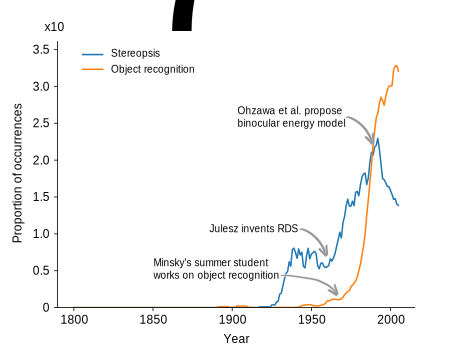
\includegraphics[keepaspectratio,width=9cm]{ngrams.pdf}
  \caption[Popularity of the n-grams `stereopsis' and `object recognition'.]{Popularity of the n-grams `stereopsis' and `object recognition'.}
  \label{fig:ch6fig1}
\end{figure}

To a non expert, figure \ref{fig:ch6fig1} might suggest that stereopsis is already well understood or that it is no longer an interesting research topic. In what follows I will argue that this is not the case. We still have a poor understanding of how different brain regions are involved stereoscopic vision. Beyond primary visual cortex, the scientific community has not yet managed to converge to a general computational framework for stereopsis, let alone designing mechanistic models that are able to predict neural responses to naturalistic 3D stimuli. Characterizing the contributions of different cortical layers is one promising line of research for exploring the interactions between different visual areas involved in stereopsis. In particular, it would be interesting to exploit the exploratory power of high-resolution functional magnetic resonance imaging to identify key circuits, which could then be dissected in greater detail using layer-specific electrical or optical recordings. The interactions between vergence, accommodation and stereopsis at the neural level are also poorly understood. There is evidence that disparity selectivity in V1 is greatly modulated by viewing distance \cite{Trotter:1992ij}, but, to my knowledge, models of disparity selectivity in V1 have yet to explain these findings.

Additionally, down-weighting the importance that studying stereopsis can have in advancing our understanding of the brain is a mistake. First, as I have mentioned before, stereopsis seems to rely on multiple brain regions across the entire brain, which attests its suitability to study how different brain regions work together to support perception. Second, stereopsis is a classical demonstration of how the brain excels at rapidly doing inverse graphics. Understanding how the brain achieves this may provide valuable insights to the fields of machine learning and artificial intelligence --- in the same way the connectionist principles inspired the development of modern, state-of-the-art artificial intelligence.


%%% ----------------------------------------------------------------------

% ------------------------------------------------------------------------

%%% Local Variables: 
%%% mode: latex
%%% TeX-master: "../thesis"
%%% End: 
